\section{Object Model}
\label{section:uml_notation}
\label{subsec:objects}

This section will cover the design choices behind the application’s object model, derived from the use cases in Section~\ref{sec:use_cases}. The UML object model diagram can be seen in Figure~\ref{fig:UML_class_diagram}, and is guided by the UML standard guide written in cooperation by several different software companies~\citep{UML_notation}.

The UML attribute notation in this report is:
\begin{itemize}
    \item PK attribute - means that the attribute is a primary key.
    \item FK attribute - means that the attribute is a foreign key.
    \item attribute : type - all attributes will have a type e.g. \verb+id : int+.
\end{itemize}

The primary purpose of \projectname{} is to connect users and drones to allow the user to interact with a drone by watching its video feed, controlling its movements or both.
Therefore the users and drones are the primary objects that must be represented in \projectname{}.\\

The system will contain the following objects and relationships:
\fxfatal{Bør Object Model snakke om Affiliate Privilege og Session?}

Objects:
\begin{itemize}
    \item User
    \item Company
    \item Role
    \item Privilege
    \item Drone
    \item Flight Plan
\end{itemize}

The relationship between the objects can be seen in Figure~\ref{fig:UML_class_diagram}.
This figure also serves as the model for the whole system.\\

\begin{figure}[htb]
    \centering
    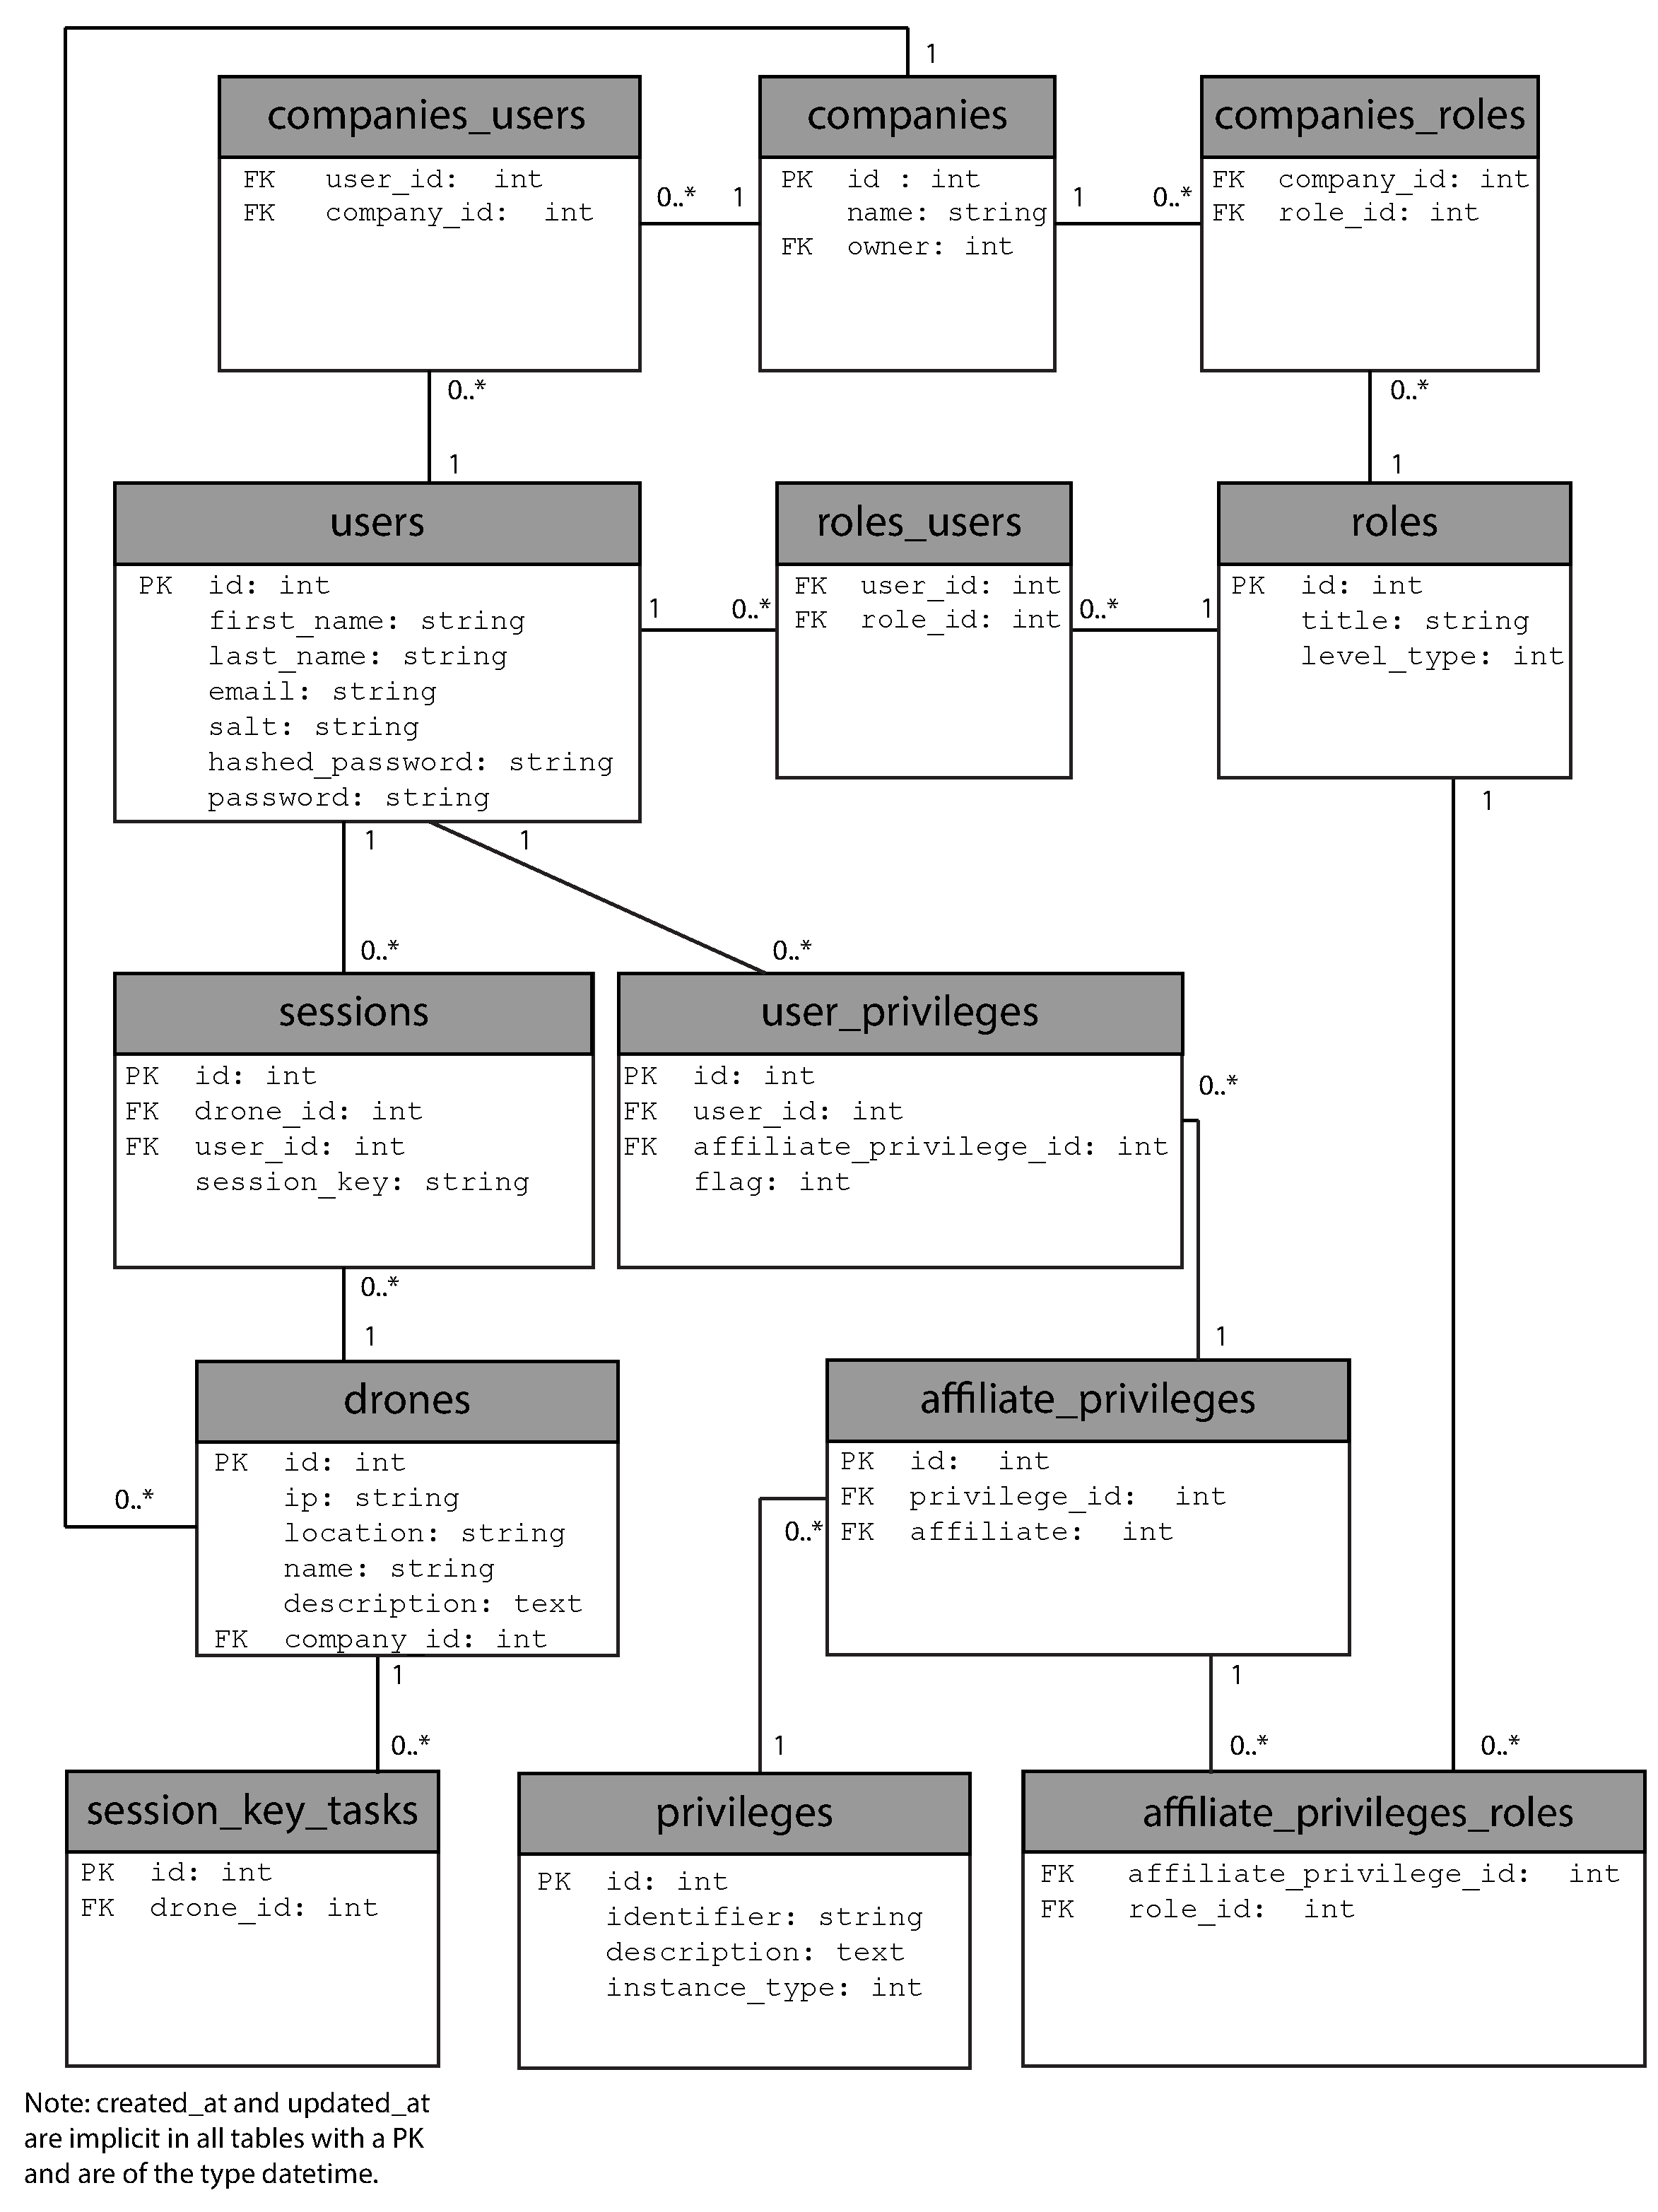
\includegraphics[width=0.95\textwidth]{gfx/UML_model.pdf}
    \caption{UML Class Diagram of \projectname{}}
    \label{fig:UML_class_diagram}
\end{figure}

The following section will analyze all the object types in the system, their relationships and why they are built as they are.
The upper part of Figure~\ref{fig:UML_class_diagram} shows the relationship between users, companies and roles/privileges while the lower part of the figure shows the relationship between drones, roles/privileges and flight plans.


\subsection{User}
Only users that are logged in with a valid username and password can interact with the system.
If you are visiting the system as a guest and hence not logged in, only a login-page will be displayed.
The system is designed so that every individual has their own unique user, allowing the system to show user-specific objects and allow user-specific access to different parts of the system. \\

A users access to the system will need to be restricted to make sure that any user only accesses what he is permitted too.
This restriction is controlled by roles and privileges.
The handling of roles and privileges will be done by the role-model. \\

A user will be identified by his e-mail address which will work as the username and therefore be unique.
Each user will also have a password, that is both salted and hashed in the database, using the SHA-1 hashing algorithm. SHA-1 has been chosen as this is considered a strong hashing algorithm that has no current or known collisions. By using a salt, the password is secured against rainbow-tables.  \\

The user-object serves as the point of entrance for anyone who wishes to use the system, and combined with companies, roles and privileges dictate its options.


\subsection{Company}
\projectname{} is designed with the intent that multiple different clients can use the system.
These clients could be different companies that in some way wishes one or more drones to surveil their premises.
One company may have several employees that they wish to provide with access to the system.
The Company-object handles this relationship, allowing multiple users to be grouped together in a company.
One User can be a member of several Company, and one Company can have many Users in it.
Therefore this is a many-to-many relationship, represented in the Companies\_users table. \\

Roles and privileges can be assigned to a Company and inherited by its Users.
This is described in further details in the following sections.


\subsection{Drone}
Along with Users, Drones are the most important object in \projectname{}.
An instance of a Drone in the system represents a physical drone somewhere in the field.
A Drone-object itself does not contain much data nor functionality.
It simply represents a drone and is a point of connection between Users and controlling the Drone itself. \\

The relationship between a User and a Drone is controlled by Privileges and Drones through Companies in most cases. \\

The logging of when a drone takes of and lands is represented by the Flightplans table.


\subsection{Flight Plan}
Flight plans are used to log whenever a drone takes of and lands and which user is issuing the commands.
One drone can have many flight plans.
One flight plan can have one drone.
Therefore this is a one-to-many relationship.


\subsection{Privilege}
\label{sec:privileges}
A Privilege-object represents a privilege that can be granted to another object in the system.
Examples of privileges are:

\begin{itemize}
    \item Add a new user to the system
    \item Edit the informations of a specific company
    \item Watch the video feed from a specific drone
    \item Control the movement of a specific drone
\end{itemize}

A privilege consists of three elements:

\begin{itemize}
    \item An action that it provides privilege to perform (such as any of the ones mentioned above)
    \item An object that these can be applied on
    \item An affiliation where the privilege is granted too.
\end{itemize}

Privileges can both be assigned directly to a user or assigned along with other privileges using a Role. \\

\projectname{} comes with a number of predefined Privileges that can be granted across the system as the administrator wishes.
But the structure of the Privileges also allows for later expansion, providing the system with scalability as more Privileges can be added to the system later without changing any of the source code of the system.


\subsection{Role}
Roles are designed to bind multiple Privileges and Users using one component to save the administrators some work.
Consider a role as a collection of Privileges that are assigned to an object in the system.
Roles can be assigned to:

\begin{itemize}
    \item Users -- in this case, it is the same as if the Privileges were granted directly to the User, only this way multiple Privileges can be assigned to a User at once.
    \item Company -- in this case, the Company administrator can assign Users in the Company to any of the assigned Roles.
\end{itemize}

As mentioned above, Roles are not the only way that a user can get a privilege granted, however.
Though a User can be granted all Privileges in a Role by getting assigned to it, a User is also able to be granted a Privilege directly via the \verb+User_Privileges+ table.


\subsection{Relationships}
The system is designed with flexibility and scalability in mind, and the structure of Roles and Privileges are what provides those features.
As described before there are two ways that a User can be granted a specific Privilege.
These are by 1) getting the Privilege granted directly via the \verb+User_Privileges+ table or 2) by being a member of a Role that via the \verb+Privileges_Roles+ table that has one or more Privileges granted.
These will be explained in details in the following subsections.


\subsubsection*{Users and Privileges}
\label{sec:users_and_privileges}
\fxfatal{Kig på subsubsections}
An administrator can grant a specific Privilege directly to a user via the \verb+User_Privileges+ table.
This Privilege is then affiliated with an object -- usually a Drone.
The Privilege could also be a system functionality, however, as described in Section~\ref{sec:privileges}. \\

This relationship is also used for exceptions.
In an example where five Users: U1, U2, U3, U4 and U5 are a member of a Role: R1, we may have a situation where U2 is not suppose to have access to a given Privilege P1 in R1.
Then a User-specific Privilege is granted to U2 on P1, but with the ``exception''-flag marked.
This is equal to blacklisting U2 from using Privilege P1, providing the system with a lot of flexibility, as even though a group of Users are granted a number of Privileges via a role, User-specific exceptions can be added to this setting. \\


\subsubsection*{Roles and Privileges}
As mentioned before -- the reason that Roles can be used to assign Privileges to a User, is to make both the administration and data structure of Users and Privileges as simple and efficient as possible.
By allowing exceptions, full flexibility is still possible. \\

This is how the relationship between Roles and Privileges works: \\

An administrator creates a Role.
Lets call this Role ``Control Drone \#4''.
A number of Privileges are assigned to this Role.
It could be the following:

\begin{itemize}
    \item Watch the video feed from a specific drone
    \item Control the movement of a specific drone
\end{itemize}

Those Privileges are then linked to this Role and to the Drone this concerns. \\

Roles can be assigned with affiliation to both Users and Companies.
Say a user \verb+U1+ needs access to Drone \#4.
User U1 then needs to either have the Privileges directly granted as described in Section~\ref{sec:users_and_privileges} or be a member of the role ``Control Drone \#4''.


\subsubsection*{Privileges and granting of Privileges}
Since it is possible to grant Privileges both directly to a User and via a Role, the same Privilege can be used in more than one context.
Therefore the \verb+Affiliation_Privileges+ table exists.
This table links the granting of a Privilege with the actual Privilege and defines on which Object the Privilege applies.
The reason for having this table and not just link the two granting-tables \verb+User_Privileges+ and \verb+Privileges_Roles+ directly to the \verb+Privileges+ table, is that we try to avoid redundant data by having the data in the \verb+Privileges+ and \verb+Affiliation_Privileges+ table make up one instance of a privilege together.
This is then granted to a User or a Role, who can then use the Privilege. \\

The system is designed so that any User can grant a Privilege he already has already been granted to another User if he is permitted to.
This is controlled via a ``re-grantable'' flag which is set in either the \verb+User_Privileges+ table or the \verb+Privileges_Roles+ table.
By marking this flag as ``true'', the User or Users that via a Role is granted the Privilege in question, can via an interface in the system re-grant the Privilege to other Users in the same Company.


%Note: Alle brugere kan videregrante et privilege hvis de har tilladelse til det. Det er et flag som sætes i user_privileges og privileges_roles, som tillader alle der har dette privilegie til at videregrante det. Husk at beskrive hvordan et privilege og et affiliation privilege til sammen giver et grant-able privilegie


\subsubsection*{Privileges and Drones}
With \projectname{} in its current form, most Privileges that are granted will have an connected with a Drone.
Privileges and its a affiliations are linked in the \verb+Affiliation_Privileges+ table.
This is also where Drones are linked to any granted privilege. \\

As described earlier, Drones are the current object-type implemented in the system.
However, the structure and model of the system allows for later expansion, connection new objects such as stationary cameras or any other type of object to the system.
The \verb+Affiliation_Privileges+ has a third field named \verb+object_id+.
This field links the Privilege, the granting of it and the Object that this granting is valid for. \\

An example could be linking Privilege P1, User U1 and Drone D1.
Say P1 is the privilege for watching the video feed of a drone.
Then the user U1 will have access to watch the video feed of Drone D1.


\subsubsection*{Drones and Flight plans}
Every time a Drone takes of or lands, it is logged to the database.
This action is logged into the \verb+Flight_plans+ table.
Each flight plan is unique and associated to only one Drone. \\

The reason for keeping this log is to enable the users of the system to later analyze the action history of any given Drone.


\subsubsection*{Drones and Companies}
The \verb+Company_drones+ table defines a relationship between a Drone and a Company.

The administrator of each Company defines the Roles in that Company.
In doing so, he defines which Privileges that are granted in every Role.
These Privileges are linked to a (Drone)-object.
The system must make sure that any Company administrator cannot link a Privilege with a Object that is not within his control. \\

This relationship defines which Drones are available to each Company.
When a Company administrator adds new Roles (and hence Privileges), he is only able to associate it with Drones that are connected to the Company in question.
